\chapter{PyMUVs}
\emph{\textbf{Py}MUVs \textbf{M}odels \textbf{U}nderwater \textbf{V}ehicle\textbf{s}}

% -----------------------------------------------------------------------------
\section{Introduction}

\pymuvs{ }is a Python library for mathematically modelling underwater vehicles. The
library is designed to be modular and easy to use, and is built on top of NumPy
\cite{numpy} and SymPy \cite{sympy}. By defining the a set of links, as well as
their properties, such as mass, inertia, volume, linear drag, quadratic drag,
external forces, and transformations between links,
\pymuvs{ }can compute a symbolic representation of the system on the
form
\begin{align}
    \bm{M}(\bm{q}) \ddot{\bm{q}} + \bm{C}(\bm{q}, \dot{\bm{q}}) \dot{\bm{q}} +
    \bm{D}(\bm{q}, \dot{\bm{q}}) \dot{\bm{q}} + \bm{g}(\bm{q}) = \bm{J}^T(\bm{q}) \bm{B} \bm{u},
    \label{eq:pymuvs:eom}
\end{align}
where the matrices $\bm{M}$, $\bm{C}$, $\bm{D}$, $\bm{g}$, $\bm{J}$, and $\bm{B}$ are
computed symbolically and can be used to simulate the system. This is especially
useful when implementing model-based controllers that require the dynamics of the
system to be on the form of, or similar to \autoref{eq:pymuvs:eom}. The library
also supports exporting the symbolic representation, and the whole model to C++
code, which can be used in real-time simulations or for significantly faster
simulations.
The library, written in Python, allows for quick and easy prototyping of
models, with the flexibility to add or remove links and transformations.
The library is open-source and can be found at
\url{https://github.com/haakonbaa/pymuvs}. 


% -----------------------------------------------------------------------------
\subsection{Motivation and Importance}

\begin{itemize}
\item Why pymuvs was created
    \begin{itemize}
    \item Gazebo can be used to simulate underwater vehicles, but it does not provide
    the model matrices needed for model-based control.
    \item Existing simulators existed, but they were either written in Rust, which
    is not as widely used as Python, or they were not as flexible as we wanted.
    \end{itemize}
\item Features
\item Assumptions
\item C++ code generation
\item The goal is to develop a controller on the eelume robot, this needs to be fast
which facilitates the development of controllers in a microcontroller environment
as well as puts restrictions
\end{itemize}

% -----------------------------------------------------------------------------
\section{Architectural Design}

\subsection{Overall Structure}

\subsection{Core Modules}

\subsection{Dependencies}

% -----------------------------------------------------------------------------
\section{Implementation details}

\subsection{Model Definition}

\subsection{Customization}

\subsection{Validation and Testing}

% -----------------------------------------------------------------------------
\section{User Guide}
\subsection{Installation}

% -----------------------------------------------------------------------------
\section{Simulator}

In addition to the \pymuvs{} library, a dedicated simulator was developed to 
model the dynamics of various underwater vehicles. The simulation results 
presented in this thesis are derived from models created using \pymuvs{}, with 
corresponding C++ code generated from these models. A custom C++ implementation 
was developed to utilize the \pymuvs{}-generated code for simulating the 
system. Throughout this thesis, this implementation is referred to as 
\textit{the simulator}.

The simulator employs the fourth-order fixed-step Runge-Kutta method, as 
described in \autoref{sec:runge-kutta}, to integrate the system dynamics. This 
method was selected due to its simplicity and reliable performance. 
Implementing the simulator in C++ offers several advantages. Firstly, C++ 
provides a highly efficient simulation environment, which is particularly 
valuable during controller design and parameter tuning. Additionally, 
controllers can be implemented directly in C++ and executed within the same 
simulation environment, an essential feature for real-time controller development.

The simulator also facilitates seamless integration with higher-level 
programming languages such as MATLAB or Python. Through C++ wrappers, 
controllers implemented in these languages can be executed alongside the 
simulation. Similarly, low-level programming languages like Rust, Go, or C can 
be compiled into shared libraries and dynamically linked with the C++ 
simulator, enabling flexible integration across different software ecosystems.

One significant benefit of using C++ is the ability to perform simulations 
faster than real-time. To demonstrate the simulator's performance, a benchmark 
test was conducted with the following parameters: a simulation time of $100 \, 
\mathrm{s}$, a time step of $\Delta t = 0.01$, and a simple PD-controller. The 
simulator successfully simulated a 3-link system with 10 states in an average 
time of $0.3757 \, \mathrm{s}$, with a standard deviation of $3.4908 \, 
\mathrm{ms}$, across 10 runs. This corresponds to a speedup factor of 
approximately $266$ times faster than real-time.

It is important to note that the mass matrix in \autoref{eq:pymuvs:eom} must be 
inverted four times per time step when evaluating $\ddot{\bm{q}}$. While the 
simulation's performance may vary based on factors such as controller 
complexity, model intricacy, and computational hardware, it is evident that the 
simulator offers a highly efficient and robust environment for dynamic system 
simulations.

% -----------------------------------------------------------------------------
\section{Conclusion}

\iffalse

\section{Modules}
The following sections will give an overview of the modules making up the
library as well as some brief examples showing basic use cases. Note that this
is not a complete overview of the library, but rather a brief introduction to
the most important functionality of each module.

% ------------------------------------------------------------------------- se3
\subsection{se3}
The \texttt{se3} module contains functions for working with the special Euclidean
group $SE(3)$. The module is built on top of \texttt{SymPy} and provides functions for
generating elements of $SE(3)$ from \texttt{SymPy} symbols, as well as functions
for computing the inverse and multiplication of the elements. A simple example
is shown below.

\begin{figure}[h]
    \centering
    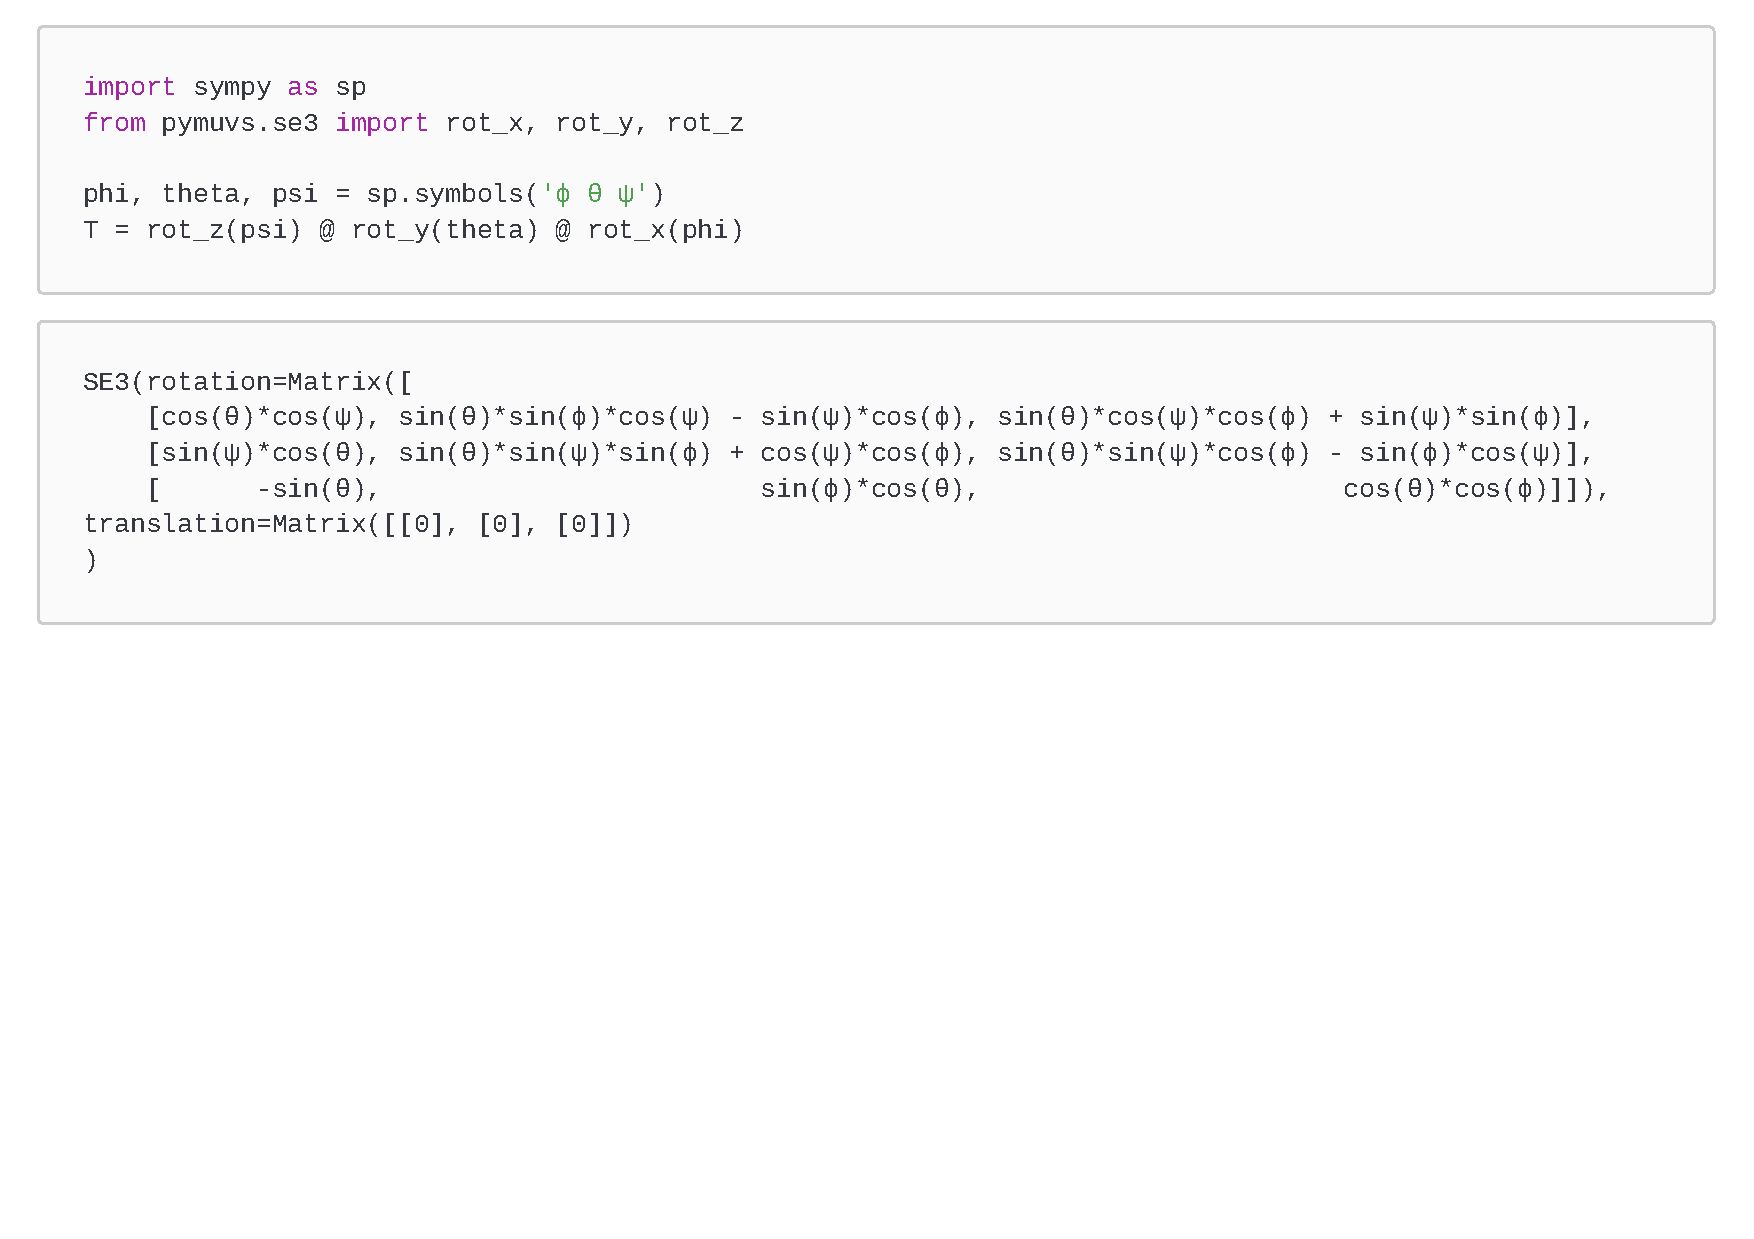
\includegraphics[page=1,width=\linewidth,trim=0 11cm 0 0]{assets/se3.pdf}
    \caption{Example usage of the \texttt{se3} module.}
    \label{fig:usage:se3}
\end{figure}

\autoref{fig:usage:se3} shows how to create a variable $T \in \SO$ representing
a pure rotation in euler angles. More elements of this class can be composed
together to form arbitrary transformations. This group is used in other modules
to represent the transformations between links in a robot model.

% --------------------------------------------------------------------- util
\subsection{util}


% --------------------------------------------------------------------- codegen
\subsection{codegen}
The \texttt{codegen} module is used to generate C++ code from a model. The module
uses the \texttt{sympy.ccode} function to generate C code from
each expression in every matrix and combines them into a header and a source
file. The \texttt{Eigen} library \cite{eigen3} is used to represent the matrices.

\begin{figure}[h]
    \centering
    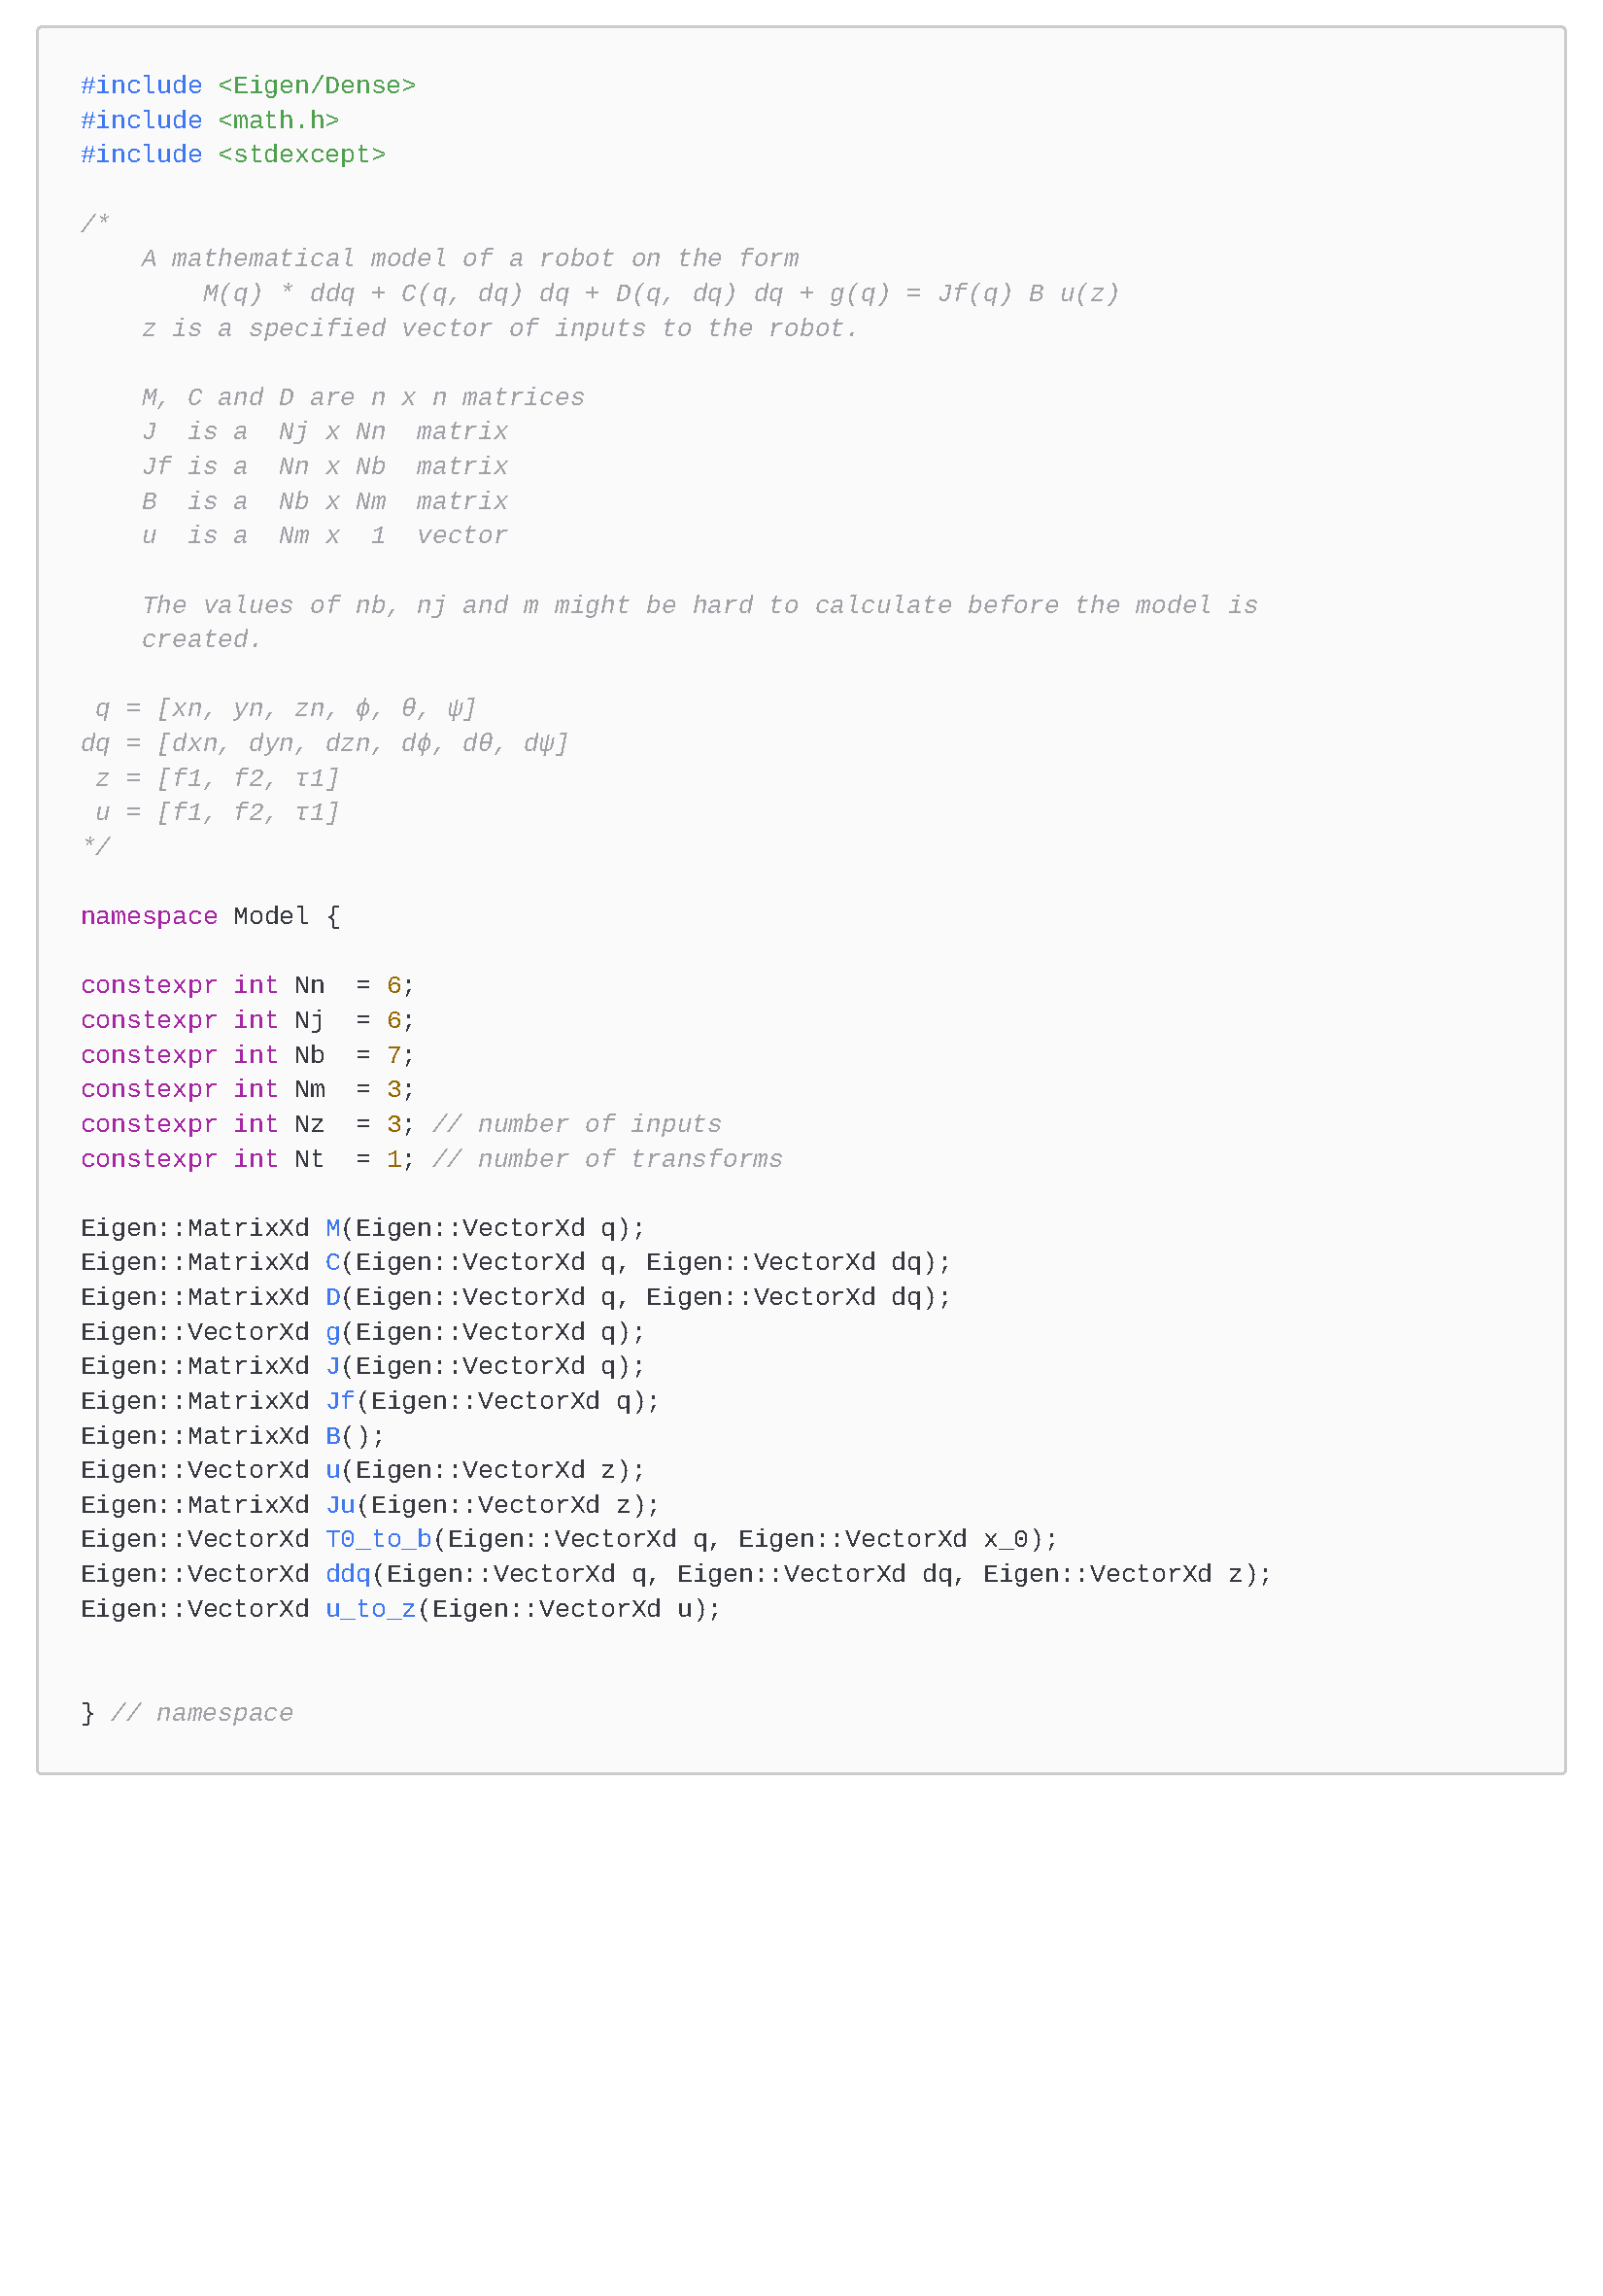
\includegraphics[page=1,width=\linewidth,trim=0 9cm 0 0]{assets/codegen.pdf}
    \caption{Automatically generated c++ code from a model.}
    \label{fig:codegen}
\end{figure}

\fi

\subsection{pymuvs}

{
    \color{red}
    \begin{itemize}
    \item masterstudent skulle lest dette og brukt PyMUVS i sin oppgave, hva trenger man å vite? (ikke detaljert dokumentasjon, bare oversikt over input/modellbeskrivelse->output)
    \item The PyMUVs chapter can be extended a bit. Sensor knows nothing about how much time you have spent on debugging and implementation, so it must be clear that this is something you have spent a lot of time on and that is an important part of your contribution.
    \item Nevn Gazebo, og at man ikke kan hente ut modellmatriser derifra, så det ikke er en fullstendig løsning for modellbasert styring av roboter.
    \item Forklar hvordan det er implementert, med matematikken bak. Stor forskjell i en prosjektoppgave på å sitere modsimboka og på å implementere en dynamisk simulator fra scratch.
    \item Beskriv hvordan systmet er definert i koden din
\end{itemize}
}
